\section*{Quality Assurance Plan}


First we need to define what \textit{QE(Qualities Ensures)}  roll will be in our software project, to understand this there is need to be defined,  this method is widely used in manufacturing industries, but its methods and terms can widely applied in software developments. When applying this methodology  it defines the standards and quality of the final software to insure that the final product becomes a high quality product.

\begin{figure}[ht!]
\centering
\includegraphics[width=90mm]{graphics/aquality.png}
\caption{Chapter 24 page 653}
\label{overflow}
\end{figure}


Quality management ensures there is a check for quality of the software during each phase of its development,  lets take into consideration the above graphic: Lest take $D(x)$ as each milestone in the waterfall method, and $Q$ as the quality management process, so in other words for each D that is complete there will be need to check $D$ and its quality requirements before proceeding to the next development phase.


By producing an accurate and well defined quality management document that includes the desire software qualities and describes how this are assessed. 

According to Humprey (1989)\footnote{Software Engineering page 653b
}, he suggest a solid structure for the quality plan, which includes:

\begin{enumerate}
	\item \textbf{Product introduction:} A description of the product, its intended market, and the quality expectations for the product.
	\item \textbf{Product plans:}The critical release dates and responsibilities for the product, along with plans for distribution and product servicing.
	\item \textbf{Process descriptions:} The development and service processes and standards that should be used for product development and management.
	\item \textbf{Quality goals:} The quality goals and plans for the product, including an identification and justification of critical product quality attributes. 
	\item \textbf{Risks and risk management:} The key risks that might affect product quality and the actions to be taken to address these risks.
\end{enumerate}


Software testing is an essential and important part of the waterfall model, which also is the main part of the quality assurance activities. In the waterfall model there may be phases which does not explicit explains the quality assurance activities, but an assurance can be included where needed in the shifts of the different phases, such as the inspections and the reviews etc..



Most of the activities in our quality assurance plan can be summarized in the model seen at left. The model illustrates the different quality assurance activities related to the waterfall model\ref{model1}\footnote{http://qatestlab.com/knowledge-center/QA-Testing-Materials/waterfall-process-in-the-quality-assurance-activities/
} and its processes. If we compare Humpreys (1989)\footnote{ Software Engineering page 653b} suggested points to the quality assurance in the waterfall model, they can be summarized to three important key characteristics:
\begin{enumerate}
	\item The testing phase, which is the main stage of the quality assurance activity.
	\item Inspections and reviews that are made and carried out at the transactions of the phases.
	\item Preventing errors especially in the early phases, and removing them during coding and testing.
\end{enumerate}

%image from testing
\begin{figure}[ht!]
\centering
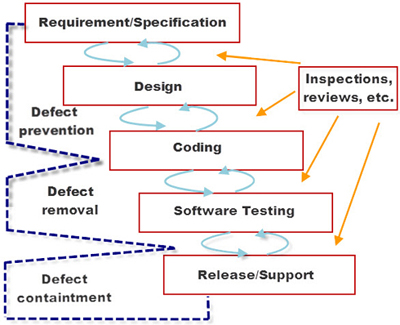
\includegraphics[width=90mm]{graphics/model1.png}{model1}
%\caption{Chapter 24 page 653}
\label{overflow}
\end{figure}

These three key point have to be implemented into the Rejse Kort project in order to make sure that the qualities are meet and lives up to what is expected. The implementation of these quality assurance activities related to the Rejse Kort system are explained below.


\subsection*{Testing phase}

In our case, we design the unit test before we start coding. After coding, the program return the results that should pass the test code. 

We also going to test the functionality, in order to do so we will use black/white box testing.

The black-box test, tests the functionality outside the software, ex. the application developed for the customers, has some intended functionalities, that we will have to ensure works properly, and doesn’t act crazy. Here we will have to create a document which specifies each test and document the outcome. On way of doing it, is to use fabricated answers, which means that we know what the result will be and then compare it against the outcome of the application.


The white-box test, tests the functionality inside the software, which means that each method, class etc. has to be tested, in order to achieve it we will have to provoke the application and see the outcome. Here we will also have to produce a document, with the specified tests, and compare it against the fabricated answers.


\subsection*{Inspections and review} 


The inspection and reviews should take place at every transaction of a phase is order to check whether the output lives up the intended result. The quality reviews will be based on documentation that are produced during the different phases, and necessarily at the software development processes. The reviews will check the consistency and completeness of what is produced during the phases in the waterfall model.


It is worth mentioning that the reviews and inspections should be tools to improve the Rejse Kort system, and not be used as tools to inspect or access the performance of the teams or the individual who are part of the process.


Our review will basically be divided into three steps in every phase:
\begin{enumerate}
	\item Pre-review activities
	\item Review meeting
	\item Post review activities
\end{enumerate}


The pre-reviews activities focuses on the review planning and preparation. Once these pre-reviews activities have been settled a review meeting can take place where the authors of a document or other \textit{“products”} being reviewed should \textit{“walk through”} or explain the \textit{“product”} with those whom are reviewing it. Once a reviewing meeting have taken place, the post review activities can take place, which handles and should address the problems and issues which were addressed at the meeting.


\subsection*{Preventing and correcting error}


The program must pass all the test code before we use it. If the program cannot pass the test code (errors and receptions ), we will use log to record it, trace the errors/receptions and fix the code. After updating the code, we test the program again and again until it can pass the test code.